\documentclass[10pt,aspectratio=169]{beamer}

\usepackage[utf8]{inputenc}
\usepackage[T1]{fontenc}
\usepackage{lmodern}
\usepackage{amsmath,amssymb,amsthm,mathtools}
\usepackage{bm}
\usepackage{xcolor}
\usepackage{tikz}
\usetikzlibrary{arrows.meta,positioning,shapes.geometric,fit,backgrounds}
\usepackage{booktabs}
\usepackage{array}

\usetheme{default}
\usefonttheme{professionalfonts}
\setbeamertemplate{navigation symbols}{}
\setbeamertemplate{footline}[frame number]
\definecolor{niceblue}{RGB}{20,40,80}
\definecolor{nicered}{RGB}{200,80,30}
\definecolor{nicegray}{RGB}{90,90,90}
\definecolor{niceboxbg}{RGB}{244,246,251}
\definecolor{niceboxrule}{RGB}{210,216,228}
\definecolor{nicegreen}{RGB}{20,110,60}
\setbeamercolor{frametitle}{fg=niceblue}
\setbeamercolor{title}{fg=niceblue}
\setbeamerfont{frametitle}{series=\bfseries,size=\Large}
\setbeamerfont{title}{series=\bfseries,size=\LARGE}
\setbeamertemplate{frametitle}{%
  \vspace*{0.5em}\insertframetitle\par
  \vspace*{-0.4em}{\color{niceblue}\rule{\textwidth}{0.5pt}}}

\newcommand{\hl}[1]{{\color{nicered}\textbf{#1}}}
\newcommand{\good}[1]{{\color{nicegreen}\textbf{#1}}}

% A real, lightly shaded rounded box used for the recurring "intuition" panels.
\usepackage{tcolorbox}
\tcbuselibrary{skins}
\newtcolorbox{ibox}[1]{%
  enhanced, sharp corners=northwest, rounded corners=southeast, arc=2.5pt,
  colback=niceboxbg, colframe=niceboxrule, boxrule=0.6pt,
  left=6pt, right=6pt, top=4pt, bottom=4pt, boxsep=1.5pt,
  fonttitle=\bfseries\color{niceblue}, coltitle=niceblue,
  title={#1}, attach title to upper, after title={\par\vspace{2pt}},
  before skip=3pt, after skip=4pt}

\newcommand{\T}{^{\!\top}}
\newcommand{\Gw}{\widetilde{G}}
\newcommand{\Mw}{\widetilde{M}}
\newcommand{\op}{\mathrm{op}}
\DeclareMathOperator{\Cov}{Cov}
\DeclareMathOperator{\Corr}{Corr}

\title{From Stationarity to Feature Geometry}
\subtitle{A residual-weighted refinement of NFA in two-layer networks}
\author{Angelo Farfan}
\date{}

\begin{document}

% ===== Slide 1: Title =====
\begin{frame}[plain]
  \vspace*{\fill}
  \begin{center}
    {\Huge\bfseries\color{niceblue} From Stationarity to Feature Geometry}\par
    \vspace{0.6em}
    {\large\color{niceblue} A residual-weighted refinement of NFA in two-layer networks}\par
    \vspace{1.0em}
    {\color{niceblue}\rule{0.55\textwidth}{0.6pt}}\par
    \vspace{1.4em}
    {\large Angelo Farfan}\par
    \vspace{0.4em}
    {May 2026 \;\textbar\; 18.S998 Final Project}\par
    \vspace{1.2em}
    {\small\color{nicegray}\texttt{github.com/elteomc/feature-learning}}
  \end{center}
  \vspace*{\fill}
\end{frame}

% ===== Slide 2: Background =====
\begin{frame}{Background: two views of feature learning}
  \footnotesize
  \begin{columns}[T,onlytextwidth]
    \begin{column}{0.48\textwidth}
      \begin{minipage}[t][0.75\textheight][t]{\linewidth}
      \textbf{NFA (Radhakrishnan et al., 2024)}\\[2pt]
      An empirical ansatz:
      \[
        B\T B \;\propto\; \mathrm{AGOP}(f)^{\alpha},
      \]
      \[
        \mathrm{AGOP}(f) = \tfrac{1}{n}\!\sum_i \nabla f(x_i)\nabla f(x_i)\T.
      \]
      Strong empirical fit. General nonlinear theory is open.
      \\[10pt]
      \textbf{FACT (Beaglehole et al.)}\\[2pt]
      First-principles move: derive a feature self-consistency identity from
      \[ \nabla_W \mathcal{L} = 0 \quad \text{at convergence.} \]
      Explains \emph{when} NFA holds and \emph{when} it can fail.
      \end{minipage}
    \end{column}
    \begin{column}[T]{0.48\textwidth}
      \begin{minipage}[t][0.75\textheight][t]{\linewidth}
      \vspace{-8pt}
      \begin{ibox}{This project: a two-layer microscope}
        Take the FACT philosophy literally in
        \[ f(x) = a\T \phi(Bx), \quad \mathcal{L} = \tfrac{1}{2n}\!\sum r_i^2 + \tfrac{\lambda}{2}\|B\|_F^2. \]
        Expand the $B$-stationarity equation. Find:
        \begin{itemize}\setlength\itemsep{1pt}
          \item the natural object is \emph{residual-weighted} AGOP, not raw AGOP.
          \item raw AGOP needs two extra links (beta, pair) which we identify and diagnose.
        \end{itemize}
      \end{ibox}
      \vspace{6pt}
      {\footnotesize\color{nicegray}
      Contribution: a finite-sample decomposition of \emph{when} raw NFA appears, \emph{which} link breaks when it fails, and a partial empirical map.}
      \end{minipage}
    \end{column}
  \end{columns}
\end{frame}

% ===== Slide 3: The question =====
\begin{frame}{What are we actually asking?}
  \begin{columns}[T,onlytextwidth]
    \begin{column}{0.48\textwidth}
      \textbf{The NFA hope}\\[4pt]
      The learned input metric $H := B\T B$ should reflect input-gradient geometry:
      \[ G \;=\; \tfrac{1}{n}\sum_i \nabla f(x_i)\nabla f(x_i)\T. \]
      \vspace{2pt}
      \emph{When is this true, and what breaks it?}
    \end{column}
    \begin{column}{0.48\textwidth}
      \vspace{-8pt}
      \begin{ibox}{The answer in this project}
        The stable late-training law is \emph{not} $H^2 \approx G$. It is
        \[ \boxed{\; H^2 \;\approx\; \kappa_{\mathrm{eff}}\, \Gw \;}, \]
        \[ \Gw = \tfrac{1}{n}\!\sum_i r_i^2\,\nabla f_i\,\nabla f_i\T. \]
        Raw AGOP appears only when an additional \emph{beta link} converts $\Gw$ into $G$, and that link becomes ill-conditioned near interpolation.
      \end{ibox}
    \end{column}
  \end{columns}
  \vspace{8pt}
  \centering
  {\small\color{nicegray}One-sentence thesis: \emph{Raw NFA is regime-dependent. The primitive object is residual-weighted.}}
\end{frame}

% ===== Slide 4: Phenomenon =====
\begin{frame}{Start with the phenomenon}
  \begin{columns}[T,onlytextwidth]
    \begin{column}{0.55\textwidth}
      \centering
      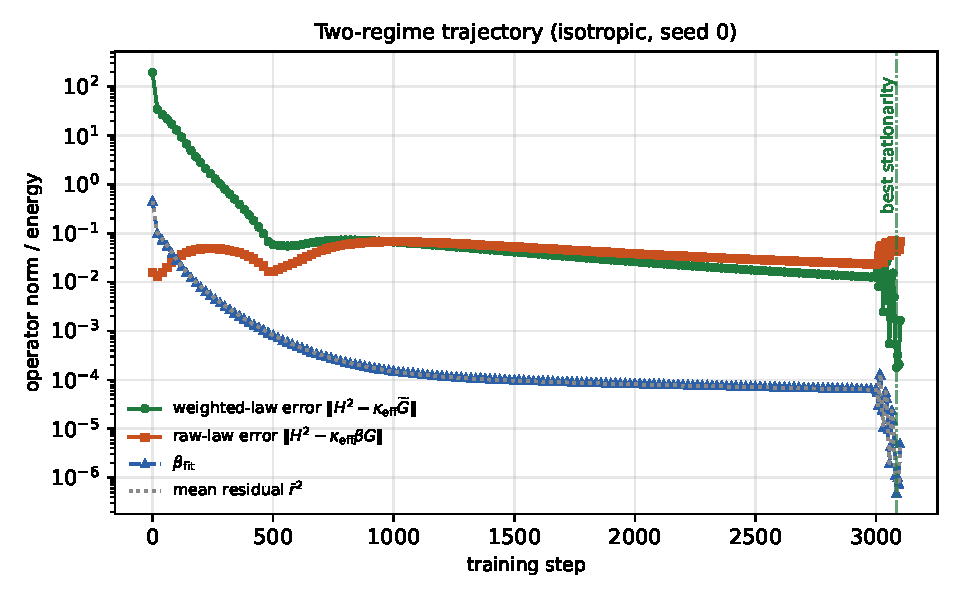
\includegraphics[width=\linewidth]{figures/two_regime_isotropic_seed_0.pdf}\\
      {\footnotesize\color{nicegray}Two-regime trajectory, isotropic seed. The step-3000 cliff is the SGD$\to$L-BFGS hand-off (see right).}
    \end{column}
    \begin{column}{0.43\textwidth}
      \footnotesize
      \textbf{What you see}
      \begin{itemize}\setlength\itemsep{2pt}
        \item Raw AGOP error (red) bottoms out in an \emph{intermediate} window.
        \item Weighted-law error (green) keeps decreasing into stationarity.
        \item Beta and mean residual energy collapse together near interpolation.
      \end{itemize}
      \vspace{5pt}
      \hl{The cliff at step 3000.} There we hand off from SGD to a stronger optimizer (L-BFGS), which breaks the SGD plateau and drives the run \emph{close to interpolation}. It is a real regime change, not a plotting glitch: as $r_i^2 \to 0$, the bridge scalar $\beta_{\mathrm{fit}}$ (a weighted average of the $r_i^2$) collapses with them, so de-weighting $\Gw \approx \beta G$ goes ill-conditioned while $H^2 \approx \kappa_{\mathrm{eff}}\Gw$ stays accurate.
      \vspace{5pt}
      \hl{Implication.} A single end-of-training correlation hides the trajectory. The weighted law is \good{stable late}, the raw law \hl{conditionally visible}.
      \vfill\null
    \end{column}
  \end{columns}
\end{frame}

% ===== Slide 5: Story map =====
\begin{frame}{The story map: two stages, not one chain}
  \centering
  \vspace{4pt}
  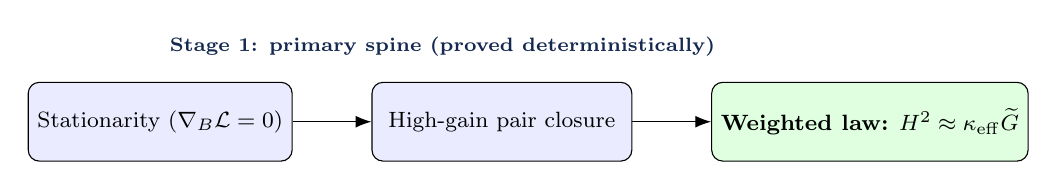
\begin{tikzpicture}[node distance=11mm, every node/.style={font=\footnotesize}]
    \node[draw, rounded corners, fill=blue!8, minimum width=29mm, minimum height=10mm] (st) {Stationarity ($\nabla_B\mathcal{L}=0$)};
    \node[draw, rounded corners, fill=blue!8, minimum width=33mm, minimum height=10mm, right=10mm of st] (pc) {High-gain pair closure};
    \node[draw, rounded corners, fill=green!12, minimum width=37mm, minimum height=10mm, right=10mm of pc] (wl) {\textbf{Weighted law:} $H^2 \approx \kappa_{\mathrm{eff}}\Gw$};
    \draw[-{Latex[length=2mm]}] (st) -- (pc);
    \draw[-{Latex[length=2mm]}] (pc) -- (wl);
    \node[above=2mm of st.north, anchor=south west, color=niceblue]{\scriptsize\textbf{Stage 1: primary spine (proved deterministically)}};
  \end{tikzpicture}

  \vspace{8pt}
  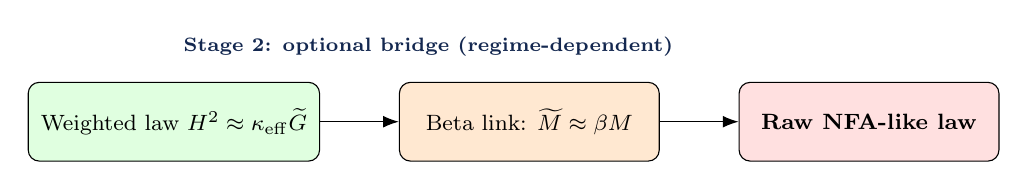
\begin{tikzpicture}[node distance=11mm, every node/.style={font=\footnotesize}]
    \node[draw, rounded corners, fill=green!12, minimum width=37mm, minimum height=10mm] (wl2) {Weighted law $H^2 \approx \kappa_{\mathrm{eff}}\Gw$};
    \node[draw, rounded corners, fill=orange!18, minimum width=33mm, minimum height=10mm, right=10mm of wl2] (bl) {Beta link: $\Mw \approx \beta M$};
    \node[draw, rounded corners, fill=red!12, minimum width=33mm, minimum height=10mm, right=10mm of bl] (raw) {\textbf{Raw NFA-like law}};
    \draw[-{Latex[length=2mm]}] (wl2) -- (bl);
    \draw[-{Latex[length=2mm]}] (bl) -- (raw);
    \node[above=2mm of wl2.north, anchor=south west, color=niceblue]{\scriptsize\textbf{Stage 2: optional bridge (regime-dependent)}};
  \end{tikzpicture}

  \vspace{12pt}
  \footnotesize
  \begin{tabular}{@{}p{0.46\textwidth}@{\hspace{4mm}}p{0.46\textwidth}@{}}
    \hl{Pair closure} fails $\Rightarrow$ \emph{weighted} law fails. &
    \hl{Beta link} fails $\Rightarrow$ \emph{only raw} law fails, weighted law is unaffected.
  \end{tabular}
\end{frame}

% ===== Slide 6: Setup =====
\begin{frame}{Setup and the key stationarity identity}
  \footnotesize
  \[ f(x) = a\T \phi(Bx), \quad r_i = f(x_i) - y_i, \quad q_i = a \odot \phi'(Bx_i). \]
  \[ X = [x_1,\ldots,x_n], \quad Q = [q_1,\ldots,q_n], \quad R = \mathrm{diag}(r_1,\ldots,r_n). \]
  \vspace{-2pt}
  \begin{columns}[T,onlytextwidth]
    \begin{column}{0.48\textwidth}
      \textbf{Loss and gradient}
      \[ \mathcal{L} = \tfrac{1}{2n}\!\sum_i r_i^2 + \tfrac{\lambda}{2}\|B\|_F^2, \]
      \[ \nabla_B \mathcal{L} = \tfrac{1}{n} QRX\T + \lambda B. \]
      \vfill\null
    \end{column}
    \begin{column}{0.48\textwidth}
      \textbf{$B$-stationarity}
      \[ \boxed{\; B = -\tfrac{1}{\lambda n} QRX\T \;} \]
      Residuals enter \emph{automatically}. They are not a modeling choice, they are the loss derivative.
      \vfill\null
    \end{column}
  \end{columns}
  \vspace{6pt}
  \begin{ibox}{Defect form (used throughout)}
    Let $Z := \lambda n B + QRX\T$. Then $Z = 0$ iff exactly stationary. We measure $\|Z\|$ at every checkpoint to quantify how close we are to the regime our theorem describes.
  \end{ibox}
\end{frame}

% ===== Slide 7: Key objects =====
\begin{frame}{The key objects, in plain language}
  \footnotesize
  \begin{ibox}{Two hidden-space matrices}
    \begin{align*}
      T \;&=\; QR^2Q\T &&\text{(weighted hidden covariance)} \\[1pt]
      S \;&=\; QRX\T X RQ\T &&\text{(same, with input pair geometry $X\T X$ inserted)}
    \end{align*}
  \end{ibox}
  \vspace{4pt}
  \begin{itemize}\setlength\itemsep{3pt}
    \item $T$ is what the residual-weighted AGOP $\Gw = \tfrac{1}{n}B\T T B$ is built from.
    \item $S$ appears \emph{automatically} from stationarity: $BB\T = \tfrac{1}{\lambda^2 n^2} S$.
    \item \hl{Pair closure} asks whether $X\T X$ acts like a scalar on the sample combinations the network actually uses:
    \[ d_{\mathrm{eff}} := \frac{\langle S, T\rangle_F}{\|T\|_F^2}, \qquad \kappa_{\mathrm{eff}} := \frac{d_{\mathrm{eff}}}{\lambda^2 n}. \]
  \end{itemize}
  \begin{ibox}{Why $d_{\mathrm{eff}}$ deserves the name ``effective dimension''}
    For isotropic $X$, $X\T X \approx d\,I$ on relevant directions, giving $S \approx d\,T$. Adaptive training instead picks out a subset of directions, so the right scalar is the data and iterate dependent $d_{\mathrm{eff}}$, not the ambient $d$.
  \end{ibox}
\end{frame}

% ===== Slide 8: Main result =====
\begin{frame}{Main result: a deterministic weighted square law}
  \footnotesize
  \begin{ibox}{Four-line derivation (intuition)}
    \vspace{-6pt}
    \begin{align*}
      \nabla_B \mathcal{L} = 0 \;&\Rightarrow\; B = -\tfrac{1}{\lambda n} QRX\T \\
      \;&\Rightarrow\; BB\T = \tfrac{1}{\lambda^2 n^2}\, S \\
      \Gw \;&=\; \tfrac{1}{n}\, B\T T B \\
      S \approx d_{\mathrm{eff}} T \;&\Rightarrow\; H^2 \approx \kappa_{\mathrm{eff}}\, \Gw.
    \end{align*}
  \end{ibox}
  \vspace{2pt}
  \begin{ibox}{Theorem (deterministic, finite-sample)}
    Under exact $B$-stationarity,
    \[
      H^2 - \kappa_{\mathrm{eff}}\, \Gw \;=\; \frac{1}{\lambda^2 n^2}\, B\T (S - d_{\mathrm{eff}} T) B.
    \]
    Hence $\|H^2 - \kappa_{\mathrm{eff}}\Gw\|_\op \le \tfrac{\|T\|_\op}{\lambda^2 n^2}\,\|B\|_\op^2 \cdot \mathcal{A}_{\mathrm{pair}}$, with $\mathcal{A}_{\mathrm{pair}} = \|T^{\dagger/2}(S - d_{\mathrm{eff}} T) T^{\dagger/2}\|_\op$.
  \end{ibox}
  \vspace{4pt}
  \hl{Important.} What actually appears in the law is the \emph{pushed} pair error $B\T (S - d_{\mathrm{eff}} T) B$, not the global $\mathcal{A}_{\mathrm{pair}}$.
\end{frame}

% ===== Slide 9: Two links =====
\begin{frame}{The two links, made precise}
  \footnotesize
  \begin{columns}[T,onlytextwidth]
    \begin{column}{0.48\textwidth}
      \textbf{Link 1. Beta stability}
      \[ \beta_{\mathrm{fit}} = \tfrac{1}{n}\sum_i \ell_i\, r_i^2, \quad \tfrac{1}{n}\sum_i \ell_i = 1. \]
      \[ \frac{\beta_{\mathrm{fit}}}{\bar r^2} - 1 \;=\; \Corr_n(\ell, r^2)\,\mathrm{CV}_n(\ell)\,\mathrm{CV}_n(r^2). \]
      \good{Holds when} hidden-gradient leverage and residual energy are weakly correlated.\\[2pt]
      \hl{Fails when} a few high-leverage samples carry systematically different residuals.\\[2pt]
      \hl{Collapses} as $r_i^2 \to 0$ near interpolation.
      \vfill\null
    \end{column}
    \begin{column}{0.48\textwidth}
      \textbf{Link 2. High-gain pair closure}\\[2pt]
      Take SVD $QR = U\Sigma V\T$. Define $G_{\mathrm{stat}} := \Sigma^2 V\T X\T$ and $F_X := V\T X\T X V - d_{\mathrm{eff}} I$. Then
      \[ B\T(S - d_{\mathrm{eff}} T) B \;=\; \tfrac{1}{\lambda^2 n^2}\, G_{\mathrm{stat}}\T F_X\, G_{\mathrm{stat}}. \]
      \good{Holds when} $F_X$ is small on the high-gain directions of $G_{\mathrm{stat}}$.\\[2pt]
      \emph{Note.} Global $\|F_X\|_\op$ can be large while the pushed error stays small. Global isotropy is a \emph{conservative} diagnostic.
      \vfill\null
    \end{column}
  \end{columns}
  \vspace{8pt}
  \begin{ibox}{One-line summary}
    Beta failure $\Rightarrow$ \emph{raw} law fails. \quad Pair failure (high-gain) $\Rightarrow$ \emph{weighted} law fails. These are different regimes.
  \end{ibox}
\end{frame}

% ===== Slide 10: Experiments setup =====
\begin{frame}{Experiments: principled diagnostics across families}
  \footnotesize
  \begin{columns}[T,onlytextwidth]
    \begin{column}{0.48\textwidth}
      \textbf{Positive families}
      \begin{itemize}\setlength\itemsep{2pt}
        \item \textbf{Isotropic Gaussian}. Clean theory regime.
        \item \textbf{Anisotropic Gaussian}. Stresses the isotropy assumption.
        \item \textbf{Low-rank signal $+$ isotropic noise}. Closer to realistic feature-learning data.
      \end{itemize}
      \vspace{4pt}
      \textbf{Adversarial families} (constructed to break a specific link)
      \begin{itemize}\setlength\itemsep{2pt}
        \item Rare hard / rare easy high-leverage clusters.
        \item Two-region gating, mixture of subspaces.
      \end{itemize}
      \vfill\null
    \end{column}
    \begin{column}{0.48\textwidth}
      \textbf{Diagnostics (theorem-aligned)}
      \begin{itemize}\setlength\itemsep{2pt}
        \item Weighted-law residual $\|H^2 - \kappa_{\mathrm{eff}}\Gw\|_\op$. \emph{Does the main law hold?}
        \item Theorem bound ratio. \emph{Is the bound meaningful?}
        \item $\beta_{\mathrm{fit}} / \bar r^2$. \emph{Does the beta link hold?}
        \item Pushed pair error $\|B\T(S - d_{\mathrm{eff}} T) B\|_\op$ vs.\ global $\mathcal{A}_{\mathrm{pair}}$.
        \item Stationarity defect $\|Z\|_\op$.
      \end{itemize}
      \vfill\null
    \end{column}
  \end{columns}
  \vspace{6pt}
  {\color{nicegray}\scriptsize Five seeds per family, best-stationarity checkpoints.}
\end{frame}

% ===== Slide 11: Experiments results =====
\begin{frame}{Experiments: what we observe (positive families)}
  \begin{columns}[T,onlytextwidth]
    \begin{column}{0.33\textwidth}
      \centering
      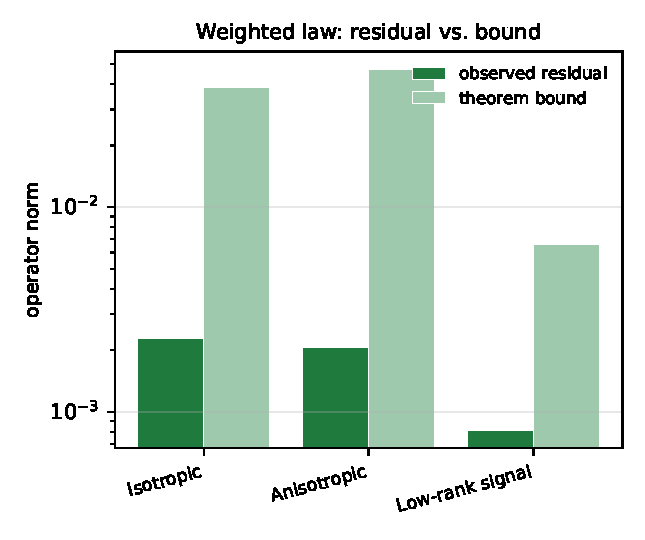
\includegraphics[width=\linewidth]{figures/weighted_law_residual.pdf}\\[2pt]
      {\footnotesize\color{nicegreen}Lower is better.\\Residual stays well under bound.}
    \end{column}
    \begin{column}{0.33\textwidth}
      \centering
      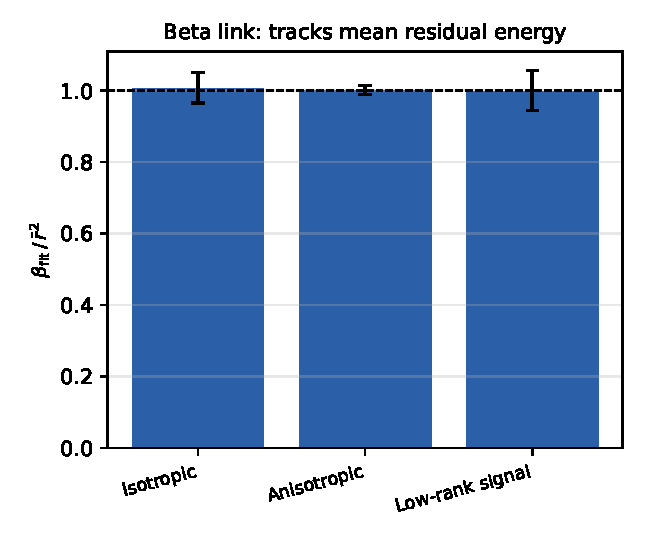
\includegraphics[width=\linewidth]{figures/beta_tracking.pdf}\\[2pt]
      {\footnotesize\color{nicegreen}Near 1 is good.\\$\beta_{\mathrm{fit}}/\bar r^2 \approx 1$.}
    \end{column}
    \begin{column}{0.33\textwidth}
      \centering
      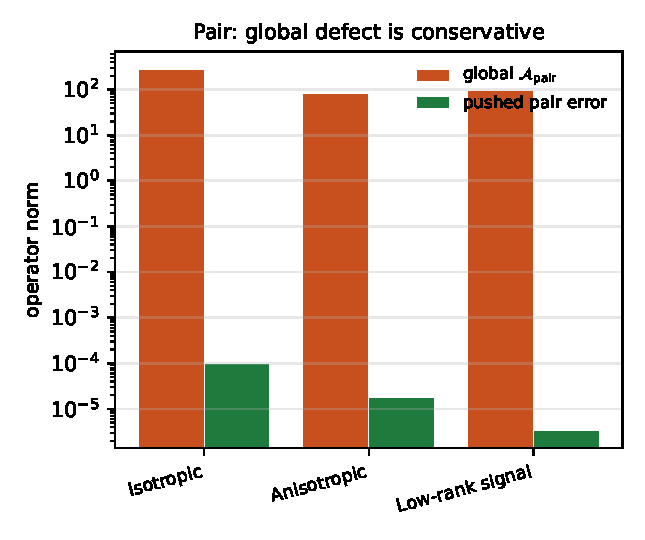
\includegraphics[width=\linewidth]{figures/pushed_pair_error.pdf}\\[2pt]
      {\footnotesize\color{nicegreen}Pushed error tiny.\\Even when $\mathcal{A}_{\mathrm{pair}}$ is not.}
    \end{column}
  \end{columns}
  \vspace{10pt}
  \footnotesize
  \begin{ibox}{Three messages}
    \begin{enumerate}\setlength\itemsep{1pt}
      \item The \good{weighted law} is accurate at best-stationarity checkpoints.
      \item The \good{beta link} holds in all three positive families ($\beta_{\mathrm{fit}}/\bar r^2 \approx 1$).
      \item Global $\mathcal{A}_{\mathrm{pair}}$ can look scary while the \good{pushed} error remains small, exactly the conservative-diagnostic scenario the theorem predicts.
    \end{enumerate}
  \end{ibox}
\end{frame}

% ===== Slide 12: Failure modes (predicted) =====
\begin{frame}{Predicted failure modes}
  \footnotesize
  \centering
  \renewcommand{\arraystretch}{1.18}
  \begin{tabular}{@{}p{4.0cm}p{4.6cm}p{4.9cm}@{}}
    \toprule
    \textbf{Regime} & \textbf{Trigger} & \textbf{Consequence} \\
    \midrule
    Beta failure (hard rare cluster)   & $\Cov_n(\ell, r^2) > 0$ large & raw law biased, weighted law fine \\
    Beta failure (easy high-leverage)  & $\Cov_n(\ell, r^2) < 0$ large & raw law biased the other way \\
    High-gain pair failure             & bad direction of $F_X$ aligns with $G_{\mathrm{stat}}$ & \hl{weighted law itself fails} \\
    Conservative pair diagnostic       & $\mathcal{A}_{\mathrm{pair}}$ large, $\|G_\mathrm{stat}\T F_X G_\mathrm{stat}\|$ small & weighted law still holds \\
    Late-regime collapse               & $r_i^2 \to 0 \Rightarrow \beta \to 0$ & raw conversion ill-conditioned \\
    \bottomrule
  \end{tabular}
  \vspace{8pt}
  \begin{ibox}{Closed-form sanity check (\texttt{run\_failure\_modes.py -{}-toy})}
    A deterministic $n = 40$ construction confirms the algebra: $\beta_{\mathrm{fit}}/\bar r^2$ moves from $\approx 1$ (balanced) to $\gg 1$ (hard rare cluster) to $\approx 0$ (easy rare cluster). The identity $\beta_{\mathrm{fit}} = \tfrac{1}{n}\sum \ell_i r_i^2$ checks to $<10^{-10}$. \emph{Next slide: a trained bridge map, and how robust the weighted law turns out to be.}
  \end{ibox}
\end{frame}

% ===== Slide 13: Trained phase diagram =====
\begin{frame}{How robust is the weighted law? A trained bridge map}
  \footnotesize
  \begin{columns}[T,onlytextwidth]
    \begin{column}{0.55\textwidth}
      \centering
      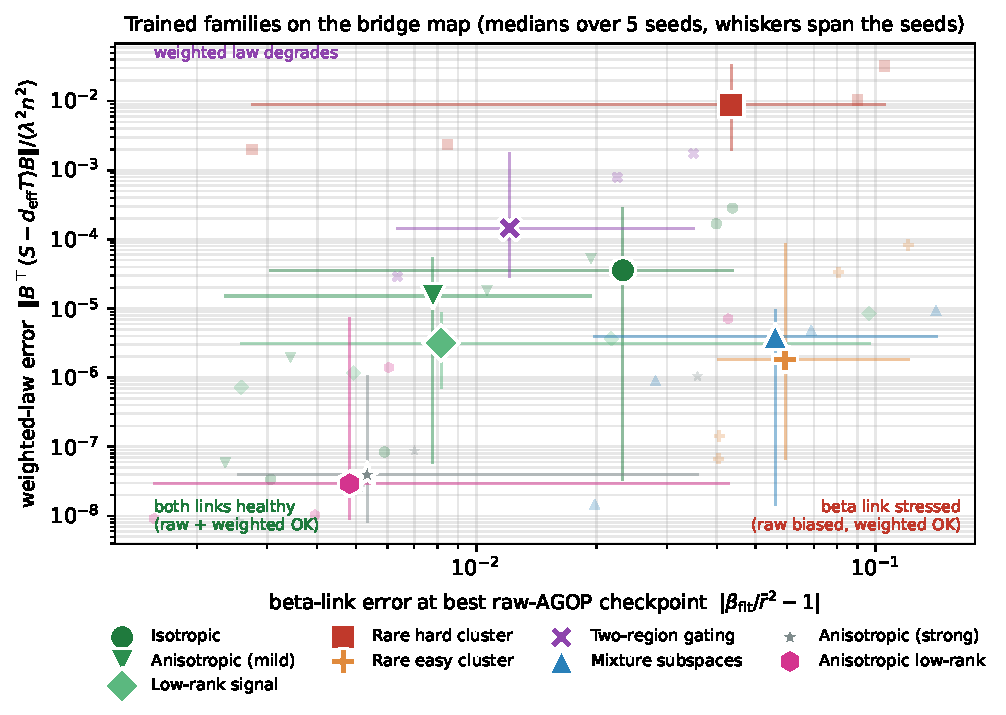
\includegraphics[width=\linewidth]{figures/phase_diagram.pdf}\\[3pt]
      {\scriptsize\color{nicegray}5 seeds per family. Marker $=$ median, whiskers span the seeds. $x$: beta-link error $|\beta_{\mathrm{fit}}/\bar r^2 - 1|$ at the best raw-AGOP checkpoint. $y$: weighted-law residual $\|B\T(S-d_{\mathrm{eff}}T)B\|/(\lambda^2 n^2)$. A guiding map, not a deliberate sweep.}
    \end{column}
    \begin{column}{0.43\textwidth}
      \begin{ibox}{What the map shows}
        \begin{itemize}\setlength\itemsep{4pt}
          \item \good{The weighted law is hard to break.} Two pair-closure attacks built on purpose (strong anisotropy, anisotropic low-rank) sit bottom-left with the positives: near stationarity the network self-aligns, so the \emph{pushed} pair error stays tiny even when global $\mathcal{A}_{\mathrm{pair}}$ is large.
          \item Mixture and rare-easy move \emph{right}: the \emph{beta} link is stressed (raw AGOP biased), the weighted law fine.
          \item Only the rare \emph{hard} cluster moves \emph{up} (two-region gating mildly): persistent amplified-outlier residuals (which also bend beta) are the one mechanism that degrades the weighted law itself.
        \end{itemize}
      \end{ibox}
    \end{column}
  \end{columns}
\end{frame}

% ===== Slide 14: Where things stand =====
\begin{frame}{Where things stand}
  \footnotesize
  \begin{columns}[T,onlytextwidth]
    \begin{column}{0.48\textwidth}
      \textbf{Proved deterministically}
      \begin{itemize}\setlength\itemsep{1pt}
        \item Exact $B$-stationarity identity.
        \item Residual-weighted square law $H^2 \approx \kappa_{\mathrm{eff}}\Gw$ with explicit error.
        \item Pushed-error factorization $\tfrac{1}{\lambda^2 n^2}G_{\mathrm{stat}}\T F_X G_{\mathrm{stat}}$.
        \item Exact beta-bridge identity $\beta_{\mathrm{fit}} = \tfrac{1}{n}\sum \ell_i r_i^2$.
        \item \hl{Bridge independence}: 2D toy instances exhibit each obstruction in isolation, so no universal NFA from stationarity alone.
      \end{itemize}
      \vspace{6pt}
      \textbf{Empirically supported}
      \begin{itemize}\setlength\itemsep{1pt}
        \item Weighted law, beta tracking, pushed-pair phenomenon (5 seeds, 3 positive families).
        \item Trained map: the beta-failure modes appear as predicted, the weighted law proves robust to pair-geometry attacks, degrading only under persistent-residual structure (rare hard cluster).
      \end{itemize}
      \vfill\null
    \end{column}
    \begin{column}{0.48\textwidth}
      \textbf{Open}
      \begin{itemize}\setlength\itemsep{1pt}
        \item \emph{Dynamics route}: derive beta decorrelation from training (leverage-sensitive damping).
        \item \emph{Adaptive concentration}: high-gain pair closure for learned subspaces.
        \item \emph{Full phase diagram}: deliberate sweeps over leverage-residual correlation and high-gain anisotropy, with samplewise diagnostics.
        \item Extension beyond two layers (layerwise Jacobian factors).
      \end{itemize}
      \vspace{6pt}
      \begin{ibox}{Take-home}
        Raw NFA is useful but \emph{regime-dependent}. The primitive object in two-layer stationarity is the \emph{residual-weighted} law, and raw AGOP is a derived consequence governed by beta and high-gain pair closure.
      \end{ibox}
      \vfill\null
    \end{column}
  \end{columns}
  \vspace{4pt}
  \centerline{\scriptsize\color{nicegray}Repo: \texttt{github.com/elteomc/feature-learning}}
\end{frame}

\end{document}
